\documentclass{report}  % Tipo de documento (puedes cambiarlo a report, book, etc.)
\usepackage[utf8]{inputenc}  % Codificación de caracteres (importante para acentos y ñ)
\usepackage[backend=biber]{biblatex}
\usepackage[scaled=1.05,proportional,lightcondensed]{zlmtt}
\renewcommand*\familydefault{\ttdefault} %% Only if the base font of the document is to be typewriter style
\usepackage[T1]{fontenc}
\addbibresource{bibliografia.bib}

\usepackage{graphicx}        % Para incluir imágenes
\usepackage{amsmath}         % Paquetes matemáticos
\usepackage{geometry}        % Configurar márgenes
\usepackage{titling}        % Configurar el título
\geometry{a4paper, margin=1in}

\title{PulpaSA}  % Título del documento
\author{Jesús Romeo Mougan}                     % Autor
\date{\today}                           % Fecha (puedes poner una fija o usar \today)

\begin{document}

\begin{titlepage}
    \newgeometry{top=3cm, bottom=3cm} % Modifica márgenes de la portada
    \centering
    \vspace*{\fill} % Empuja el contenido hacia el centro

    %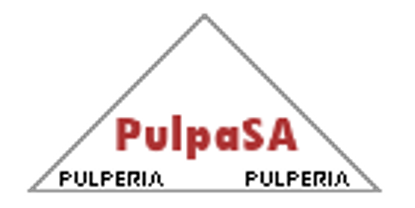
\includegraphics[width=0.5\textwidth]{images/image.png} 
    %\vspace{2cm}

    {\Huge \textbf{\thetitle}} \\[1cm]
    {\large Game Design Document} \\[1.5cm]

    \vspace*{\fill}

    {\large \textbf{\theauthor}} \\ [1cm]
    {\large IES San Clemente} \\[4cm]

    \vspace*{\fill} % Empuja hacia la parte inferior

    {\large \today}

    \restoregeometry % Restaura los márgenes normales para el resto del documento
\end{titlepage}



% cambiar Contents por Índice
\renewcommand{\contentsname}{Índice}

\tableofcontents

\newpage

\section{Introducción}
fds
\normalfont {Esto es un texto normal.}
\newline

Aquí empieza el contenido de mi documento en \LaTeX.
\newline
s
\section{Ejemplo de Ecuaciones}
Podemos escribir ecuaciones matemáticas como estafdsds
\[
    E = mc^4
\]

\section{Conclusión}
Este es un documento sencillo en \LaTeX.

\end{document}
